\section{Background}

\Glspl{GWAS} have found a number of \glspl{SNP} in the \gene{IL2RA} gene on chromosome 10 that associate with T1D.
The \gene{IL2RA} gene codes for the alpha chain of the trimeric \protein{IL-2} cytokine receptor, also known as \protein{CD25},  
which is found at varying quantities on the surface of numerous T lymphocyte subsets such as naive, memory and
regulatory cells.
\protein{CD25} is upregulated upon activation in many cells, including certain innate immune cell subsets,
and is known to play a key role in immunoregulation and immune responsiveness \citep{Brusko:2009bn,Boyman:2012cy}.
Further fine-mapping of \gene{IL2RA} by \citet{Lowe:2007ij}, \cite{Smyth:2008kx} and \cite{Maier:2009hh}, has yielded three SNPs, two of which lie within
the first intron of \gene{IL2RA}:
\begin{itemise}
  \item \snp{rs12722495}  
    %juvenile idiopathic athritis
  \item \snp{rs2104286}, also protective for multiple sclerosis \citep{Beecham:2013hh}
  \item \snp{rs11594656}, also protective for rheumatoid arthritis \citep{Stahl:2010dy}
\end{itemise}


To better study the downstream implications of these SNPs on \protein{CD25} expressing T lymphocyte 
%(Figure~\ref{figure:lymphocyte-subsets})
subsets, \citet{Dendrou:2009dv} selected samples obtained from healthy donors
chosen by genotype at these SNPs, age and sex from the CambridgeBioresource\footnote{\url{www.cambridgebioresource.org.uk}}.
The experiment consisted of a total of $180$ individuals, sixteen of which were recalled for a second sample (Table~\ref{table:IL2RA-recalled-individuals}).
%A total of 224 FCS files.
%and split into to seven genotype groups.
The distribution by age ($20$ to $50$ years old) and sex is split evenly across genotype groups.  
The running time of the whole experiment was seven months over which samples were analysed on $51$ days,
between one and eight samples per day (Figure~\ref{figure:IL2RA-sample-time}).  

The cell phenotypes studied by \citet{Dendrou:2009dv}, were obtained using manual gating with the FlowJo software\footnote{\url{www.flowjo.com}}.
Manual gating follows the current state of understanding of immune cell lineages (Figure~\ref{figure:manual-gating-strategy}).
Lymphocytes are distinguishable from more granular and larger cell types based on forward and side scatter.
Within the lymphocytes, the subset expressing \protein{CD4} are defined as T lymphocytes.
The CD4+ T lymphocyte subset can be further divided into regulatory and non-regulatory cells (Figure~\ref{figure:manual-gating-strategy}c).
Regulatory cells represent a lower frequency subset which are higher in \protein{CD25} and lower in \protein{CD127}.
Regulatory T cells can be defined more precisely by an internal marker on the \protein{FOXP3} transcription factor.
Non regulatory T cells represent the bigger proportion of T lymphocytes.
They express more \protein{CD127} and less \protein{CD25} than regulatory T cells.
The non regulatory T cells can be further divided into naive and memory subsets (Figure~\ref{figure:manual-gating-strategy}d).
Naive and memory are transitional cell populations because naive cells are activated into memory cells upon antigen presentation.
Typically as a result of this activation, the \protein{CD45RA} is lost so that consequently naive cells are higher in CD45RA than memory cells.
A further secondary distinguishable property is that memory cells tend to be higher in \protein{CD25} expression than naive cells.
Since \protein{CD25} expression on the naive cells is low, \citet{Dendrou:2009dv} define a threshold above which naive cells are deemed positive on CD25.
Their threshold is defined in terms of an isotype control, a sample not stained for \protein{CD25}, to measure the background.
%adjusted depending on the MFI of the blank beads population on that day.

Since samples were collected and analysed over a period of seven months, 
instrument variation is detectable in the CD25 mean fluorescence intensity (MFI) of the memory cell population (Figure~\ref{figure:memory-CD25MFI-time-effect}).
To correct for this time effect, beads are ran daily in order to define a transform from MFI to molecules of equivalent
fluorescence (MEF).
These beads can also be used to define a threshold above which naive cells are considered positive for \protein{CD25}.
The bead data consists of six populations which are manually gated by \citet{Dendrou:2009dv}.
In the first section of this chapter, my first task will be to gate the bead data automatically.
Next I will move on to the automatic gating of cell phenotypes.
% Calli's results
% cell phenotypes
\citet{Dendrou:2009dv} assessed the repeatability of the cell phenotypes and tested for association with genotype, sex and age.
Their results are summarised in Table~\ref{table:calli-results}.  
The objective of this chapter will be to assess whether I can replicate or improve on these results by replacing manual gating by a computational method.
Ideally the entire manual gating process should be replaced by an automatic algorithm.
But in order to facilitate initial comparison with manual gating, in this chapter,
I will only automate the two last univariate gating steps (Figure~\ref{figure:manual-gating-strategy}d):
\begin{itemise}
\item On \protein{CD25} to threshold naive cells into positive and negative subsets.
\item On \protein{CD45RA} to identify naive and memory cells within a two population mixture.
\end{itemise}

\clearpage

\begin{figure}
\centering
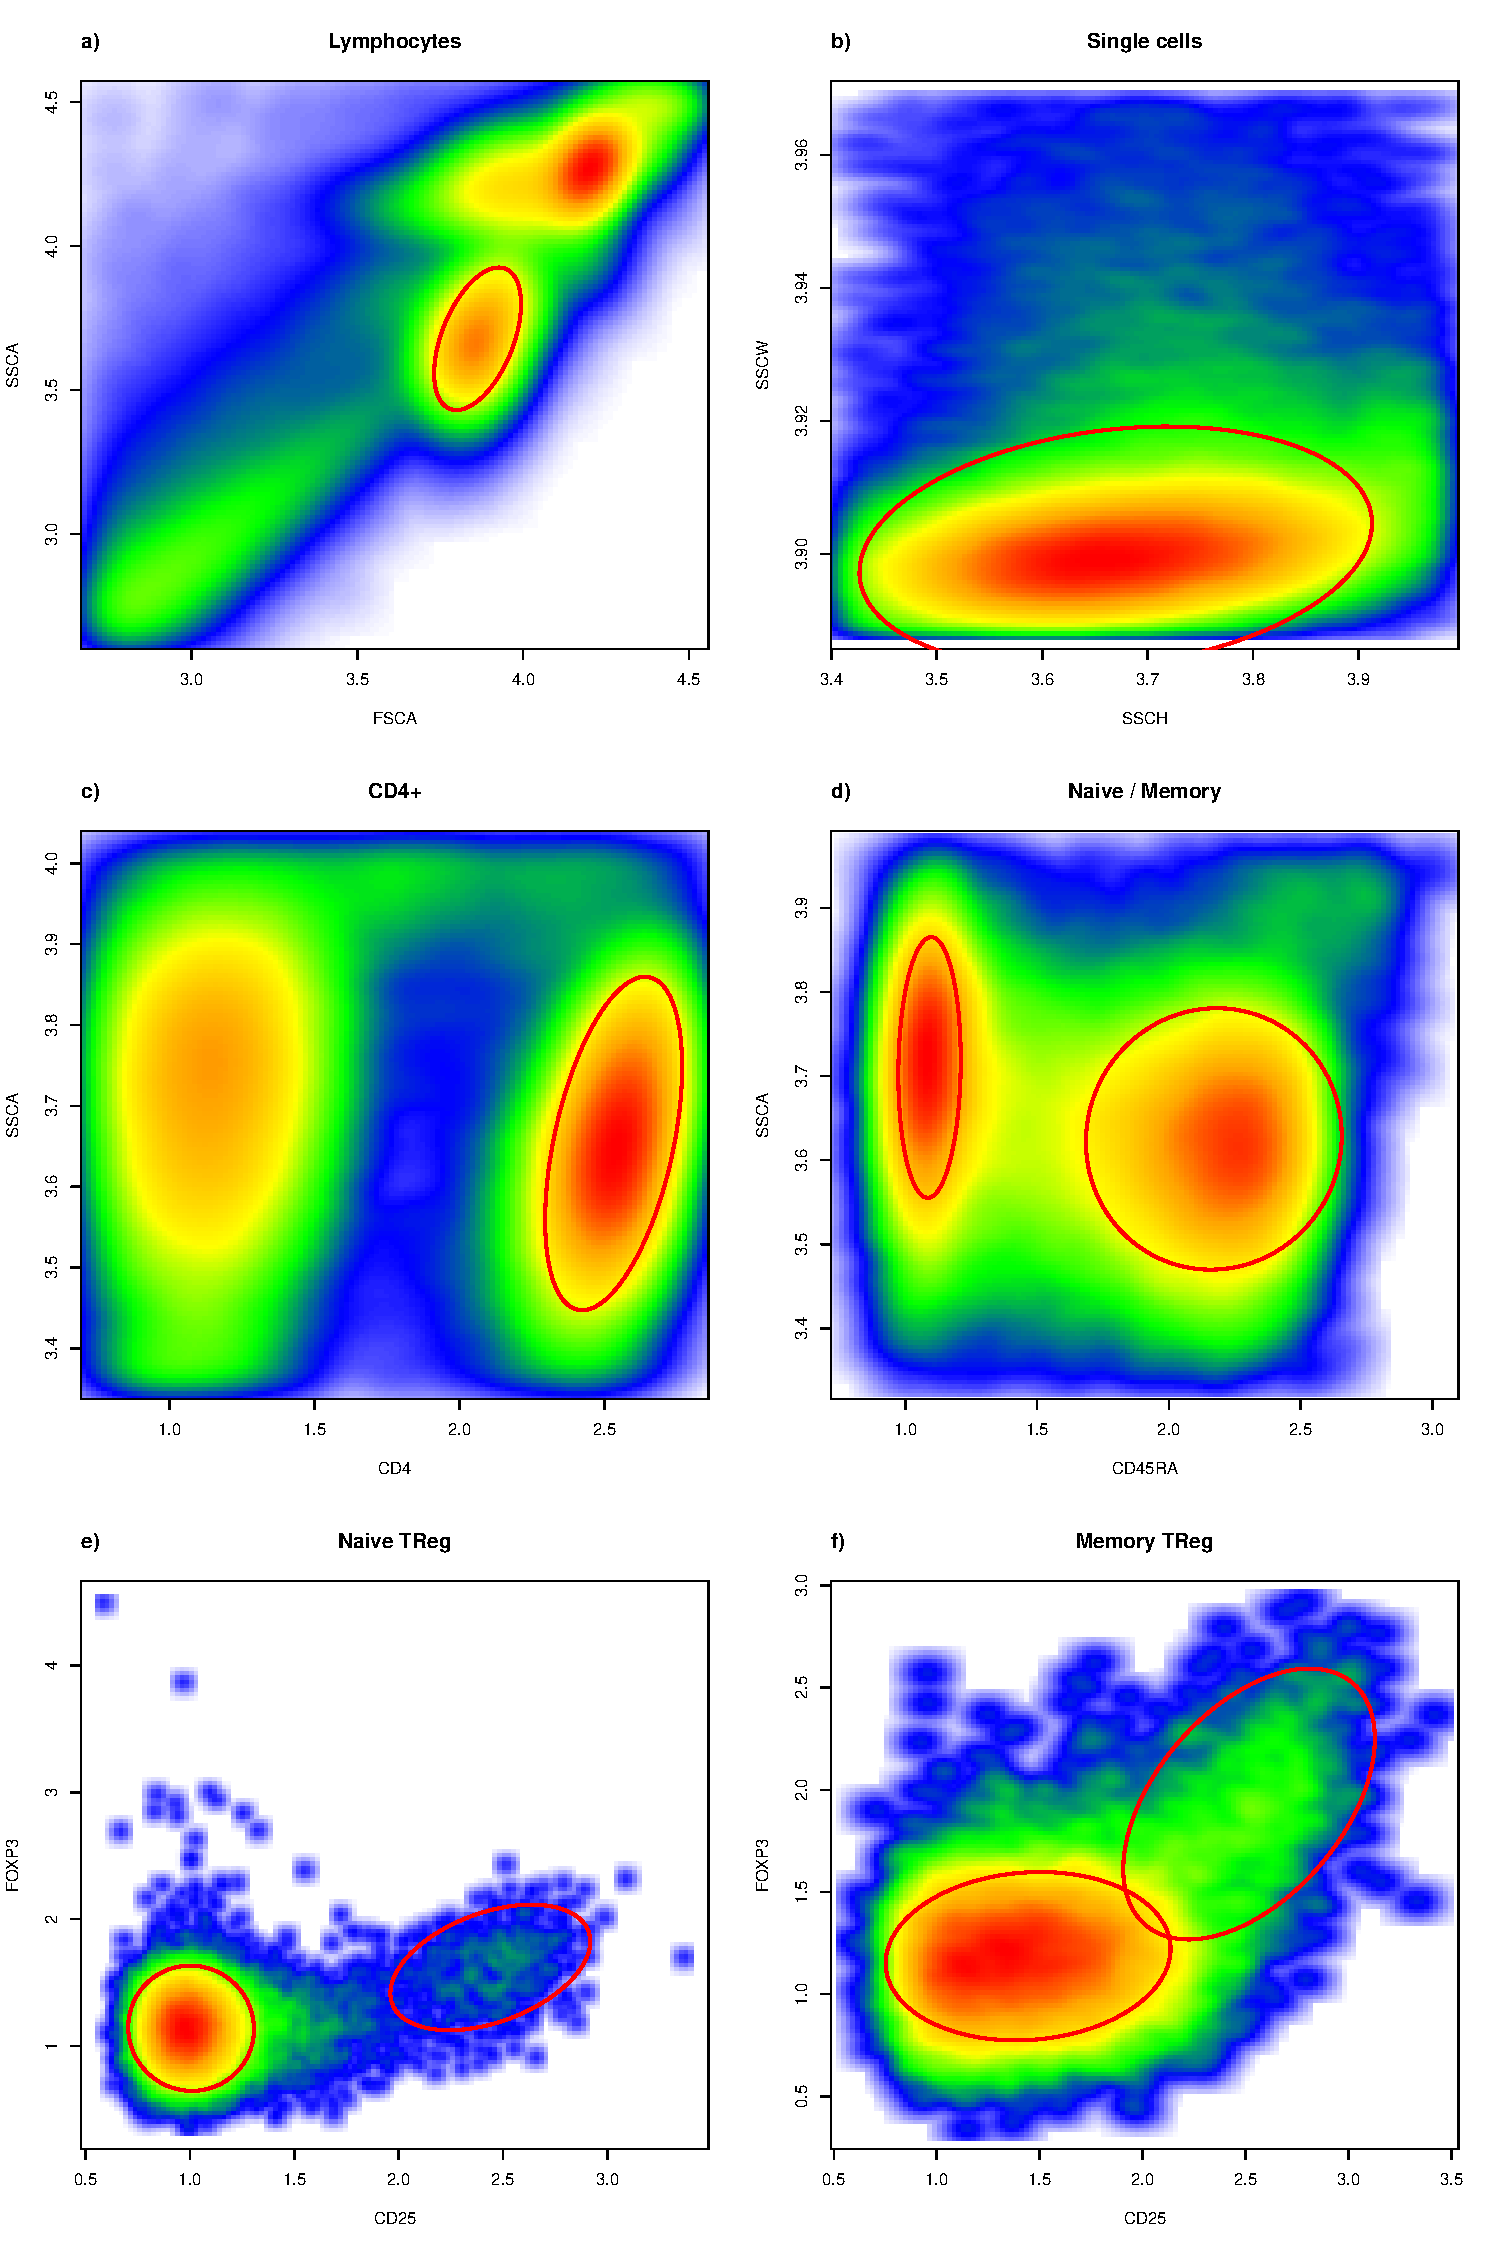
\includegraphics[scale=.5] {IL2RA/figures/ManualGating/manual-gating.pdf}
\caption{
\label{figure:manual-gating-strategy} 
%\textbf{Manual gating of IL2RA dataset.}
Manual gating strategy to extract memory T cells and CD25+ naive T cells (green boxes).
Note that the CD45RA gates exclude cells which are considered to be neither memory nor naive.
Our automated gating replaces the final stage of the manual gating on CD25 and CD45RA.
}
\end{figure} 

\begin{table}[ht]
\centering
\begin{tabular}{lc}
\rowcolor{Gray}
Flurochrome  & \\
Alexa-488    & CD127\\
PE-Cy7       & HLADR\\
APC          & CD25\\
PE           & CD101\\
Alexa-700    & CD4\\
Pacific Blue & CD45RA\\
\end{tabular}
\caption{
\label{IL2RA-panels}
The fluorochrome-antibody panels with six markers used in the ILRA dataset.
%Subset of the fluorochrome-antibody panel used by \citet{Dendrou:2009dv} to identify non T regs in whole blood
}
\end{table}

%CD101,CD127,CD25_MA251+2A3,CD4,CD45RA,HLADR
%CD127,CD25_MA251+2A3,CD4,CD45RA,ISO 

\begin{figure}
\centering
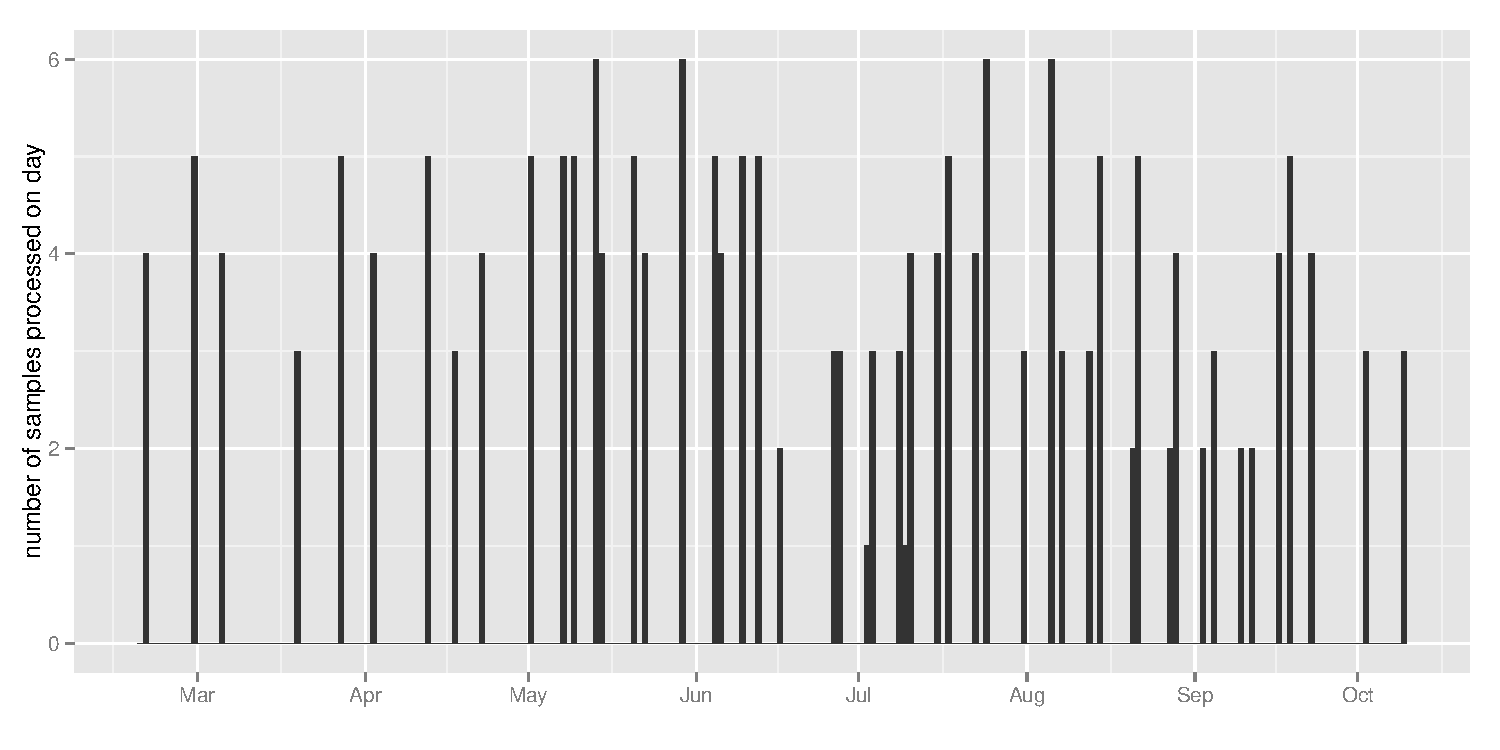
\includegraphics[scale=.5] {flowdatasets/figures/il2ra-samples-time.pdf}
\caption{
\label{figure:IL2RA-sample-time} 
\textbf{Number of samples analysed per day.}
A total of 224 samples were analysed over seven months (from March to October).
During that period, samples were analysed on $51$ days,
with between one and eight samples analysed each day.
}
\end{figure}

\begin{table}[ht]
\centering
\begin{tabular}{lllllll}
  \hline
         & individual & pch & day1       & day2       & day diff \\
  \hline
  1      & CB00058M   & a   & 2008-03-04 & 2008-09-16 & 196 \\
  2      & CB00427N   & b   & 2008-02-20 & 2008-10-02 & 225 \\
  3      & CB00435X   & c   & 2008-02-28 & 2008-10-02 & 217 \\
  4      & CB00459Y   & d   & 2008-03-26 & 2008-10-09 & 197 \\
  5      & CB00470K   & e   & 2008-04-10 & 2008-09-18 & 161 \\
  6      & CB00474P   & f   & 2008-04-16 & 2008-09-16 & 153 \\
  7      & CB00475Q   & g   & 2008-05-08 & 2008-09-18 & 133 \\
  8      & CB00496N   & h   & 2008-05-12 & 2008-09-22 & 133 \\
  9      & CB00503W   & i   & 2008-05-06 & 2008-09-18 & 135 \\
  10     & CB00555C   & j   & 2008-05-22 & 2008-09-16 & 117 \\
  11     & CB00563L   & k   & 2008-05-29 & 2008-09-18 & 112 \\
  12     & CB00566P   & l   & 2008-05-29 & 2008-09-18 & 112 \\
  13     & CB00568R   & m   & 2008-05-29 & 2008-09-22 & 116 \\
  14     & CB00588N   & n   & 2008-06-12 & 2008-10-09 & 119 \\
  15     & CB00591R   & o   & 2008-06-16 & 2008-09-22 & 98 \\
  16     & CB00646B   & p   & 2008-07-15 & 2008-10-02 & 79  \\
  \hline
\end{tabular}
\caption{
\label{table:IL2RA-recalled-individuals}
\textbf{Recalled indiviuals.}
Sixteen individuals recalled between 79 and 226 days later.
}
\end{table}

\begin{figure}[h]
\centering
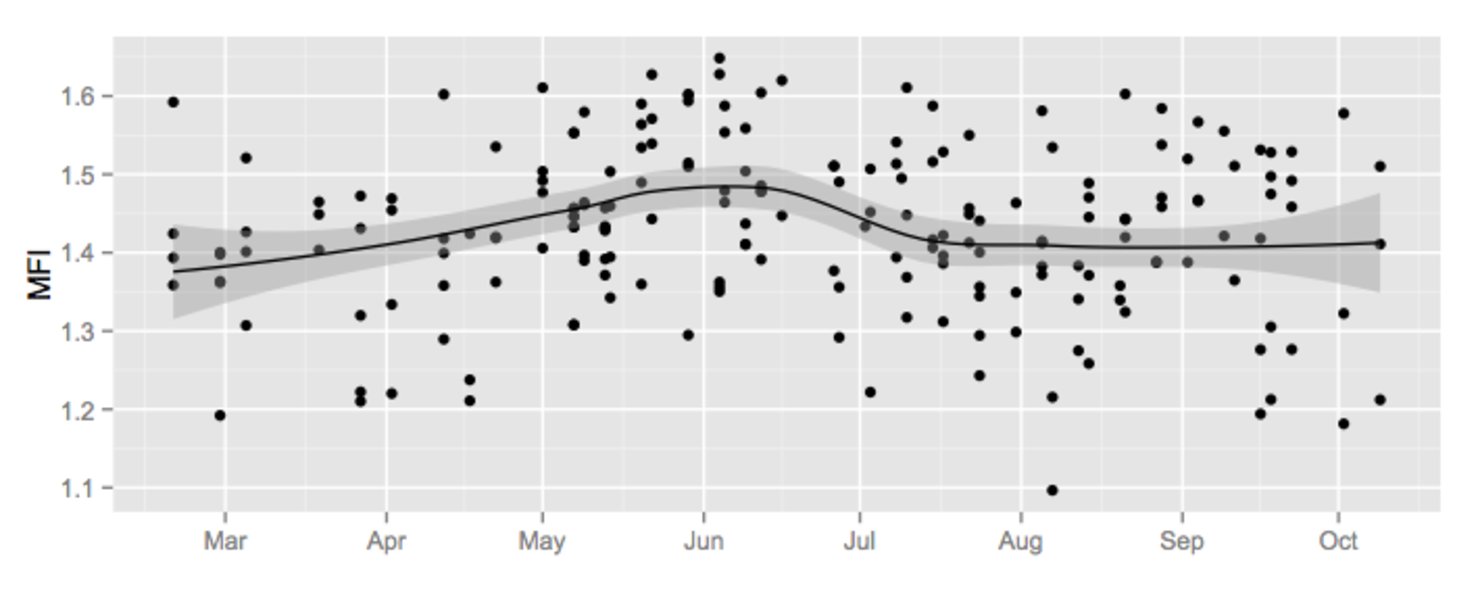
\includegraphics[scale=0.6]{IL2RA/figures/CD25-mfi-time-effect.pdf}
\caption{
\label{figure:memory-CD25MFI-time-effect}
\textbf{Effect of time on CD25 MFI in memory cells.}
\protein{CD25} MFI of memory cell population (manually gated) over time of experiment.
The black line represents the loess regression line.
}
\end{figure}


\begin{table}[hb]\footnotesize
\begin{tabularx} {\linewidth} {|XlcXXX|}
\cline{1-6}
\mbox{CD4+ T Cell} Subset & Phenotype  & Repeatability ($r^2$) & Genetic Effect                                                            & Age Effect                                & Sex Effect\\
\cline{1-6}
CD25+ Naive               & Percentage & $0.669$               & \mbox{$\downarrow$ \snp{rs2104286}} \mbox{$\text{P}=4.25 \times 10^{-6}$} & $\uparrow$ \mbox{$P=2.22 \times 10^{-9}$} & \mbox{M < F} \mbox{$P=0.005$}\\
\cline{1-6}
Memory                    & CD25 MEF   & $0.997$               & \mbox{$\uparrow$ \snp{rs12722495}} \mbox{$\text{P}=1.16 \times 10^{-10}$} & None                                      & None \\
\cline{2-6}
                          & Percentage & $0.997$               & None                                                                      & $\uparrow$ \mbox{$P=8.97 \times 10^{-5}$} & None \\
%CD4+ FOXP3+ T Cells
%CD25 MEF
%Percentage
\cline{1-6}
\end{tabularx}
\caption{
\label{table:calli-results}
\textbf{Repeatability and effect sizes of percentage of naive \protein{CD25}+, \protein{CD25} MEF and percentage of memory cell phenotypes.}
Subset of results from \citet{Dendrou:2009dv} for cell populations under re-analysis in this chapter.
$r^2$ is the Pearson correlation squared.
}
\end{table}



%%% BEADS
\section{Univariate clustering of bead data}

In flow cytometry, a method of normalising fluorescence intensity to account for instrument variation, is to convert Mean Fluorescence Intensity (MFI)
to Molecules of Equivalent Fluorochrome (MEF) \citep{Schwartz:1996jj,Dendrou:2009bl}.
In order to apply this conversion, specially designed beads of known and (assumed) constant fluorescence defined in terms of MEF are used as a reference.
The MEF property of these beads is deemed stable whereas the MFI of the bead population is dependent on the instrument and varies over time.

The beads we use are specially manufactured so that they belong to six distinct populations of increasing MEF as shown in Table~\ref{table:fluorospheres}.
Following the bead manufacturer's guidelines, plotting the $\log_{10}(MEF)$ of these six bead populations against
the corresponding calculated $\log_{10}(MFI)$ from the gated bead populations, we fit the linear regression:

\begin{equation}
    \log_{10}(\text{MEF})=\beta \times \log_{10}(\text{MFI}) + \alpha
\label{equ:MEF}
\end{equation}

The MEF is in fact a power transform of the MFI\footnote{This transform is only defined for strictly positive MFI values}:

\[
    \text{MEF}= 10^\alpha \times \text{MFI}^\beta
\]

The original MEF transform used by \citet{Dendrou:2009bl} assumes that $\beta=1$ which
gives similar results given that I found that the $\beta$ term in Equation~\ref{equ:MEF} turns out to be on average $0.96$.

In estimating the parameters slope parameter $\beta$ and the intercept $\alpha$ of the linear model,
only the non blank beads are used because the MEF of the blank beads is not specified by the manufacturer.
In fact extrapolating the MEF of the blank beads yields the detection threshold (Figure~\ref{figure:mef}) which we will see in the next section,
can be used as a threshold to define a positive cell subset.
The MEF of the blank beads is always greater than the intercept $\alpha$  which represents the log offset (the zero channel value).
%Below this threshold the intensity is meaningless as the blank beads contain by design no fluorochrome.

Typically bead data is gated manually \citet{Dendrou:2009bl}.
Here, in order to obtain the parameters of the MEF transform, I will use an automatic process to gate the beads.

Because all beads are known to be of identical shape and size, we expect a single cluster in the scatter channels: the singlet bead population.
Events which lie away from the singlet population are deemed to be beads clumped together or debris and so are discarded.
Filtering of singlets can be achieved by fitting a bivariate normal distribution on forward and side scatter and only keeping the 95th percentile.
Having gated the singlets, I subset the data and proceed to gate on the fluorescence channels to identify the six bead populations.
Given that the number of bead populations is known, that the bead signal is clean and that the number of events is small (in the order to 10,000),
I use the K-medoid algorithm (Appendix~\ref{appendix:clustering}).
The solution has been implemented in the \Rpackage{flowBeads} R package.
Automatic gating shows near perfect agreement with manual gating (Figure~\ref{figure:bead-agreement}) and so is now the established method of analysing
bead data in our lab.
Applying the bead normalisation to the memory CD25 MFI from Figure~\ref{figure:memory-CD25MFI-time-effect}, we improve on the repeatability of that 
cell phenotype from $r^2=0.629$ to $r^2=0.937$ (Figure~\ref{figure:CD25-MFI-beads-normalised}).

\clearpage

\begin{table} [hb]
\begin{center}
\begin{tabular} {|c c c c c c|}
\cline{1-6}
Population  & FITC    & RPE     & REP-Cy5 & \textbf{APC}     & PE-Texas Red\\
\cline{1-6}
1           & B       & B       & B       & \textbf{B}       & B \\
2           & 2,500   & 1,500   & 750     & \textbf{4,100}   & 552\\
3           & 6,500   & 4,400   & 2,100   & \textbf{10,300}  & 2,014\\
4           & 19,000  & 14,500  & 6900    & \textbf{25,500}  & 6,975\\
5           & 55,000  & 43,800  & 22,100  & \textbf{67,300}  & 20,685\\
6           & 150,000 & 131,200 & 77,100  & \textbf{139,100} & 71,888\\
\cline{1-6}
\end{tabular}
\end{center}
\caption{
\label{table:fluorospheres}
\textbf{FluoroSpheres from DakoCytomation.}
The Molecules of Equivalent Fluorochromes (MEF) values for the six bead populations as provided by the manufacturer.
B denote the blank beads which by design contain no fluorochrome.
Of the six fluorochromes contained by each bead only APC is used in the experiment.
}
\end{table}

\begin{figure}[hb]
\centering
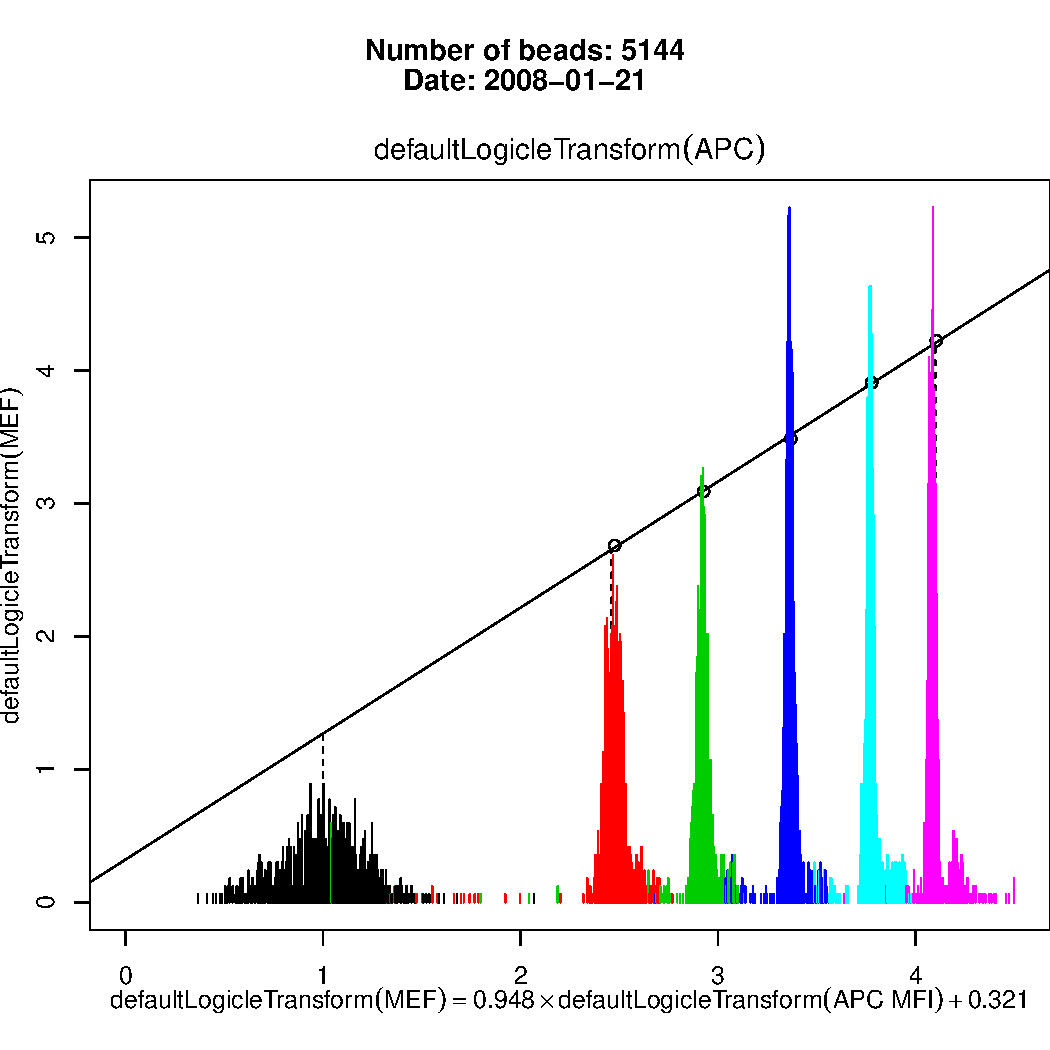
\includegraphics[scale=.5]{IL2RA/figures/Beads/flowBeads.pdf}
\caption{
\label{figure:mef}
Linear regression of bead APC MFI against the APC MEF as defined in Table~\ref{table:fluorospheres}.
The six peaks represent the six bead populations.
%The horizontal dash lines represent the MEF of the six bead populations.
%The red and green vertical lines define the range of memory CD25 MFI across all samples in \citet{Dendrou:2009dv}.
}
\end{figure}


\begin{figure}[hb]
\centering
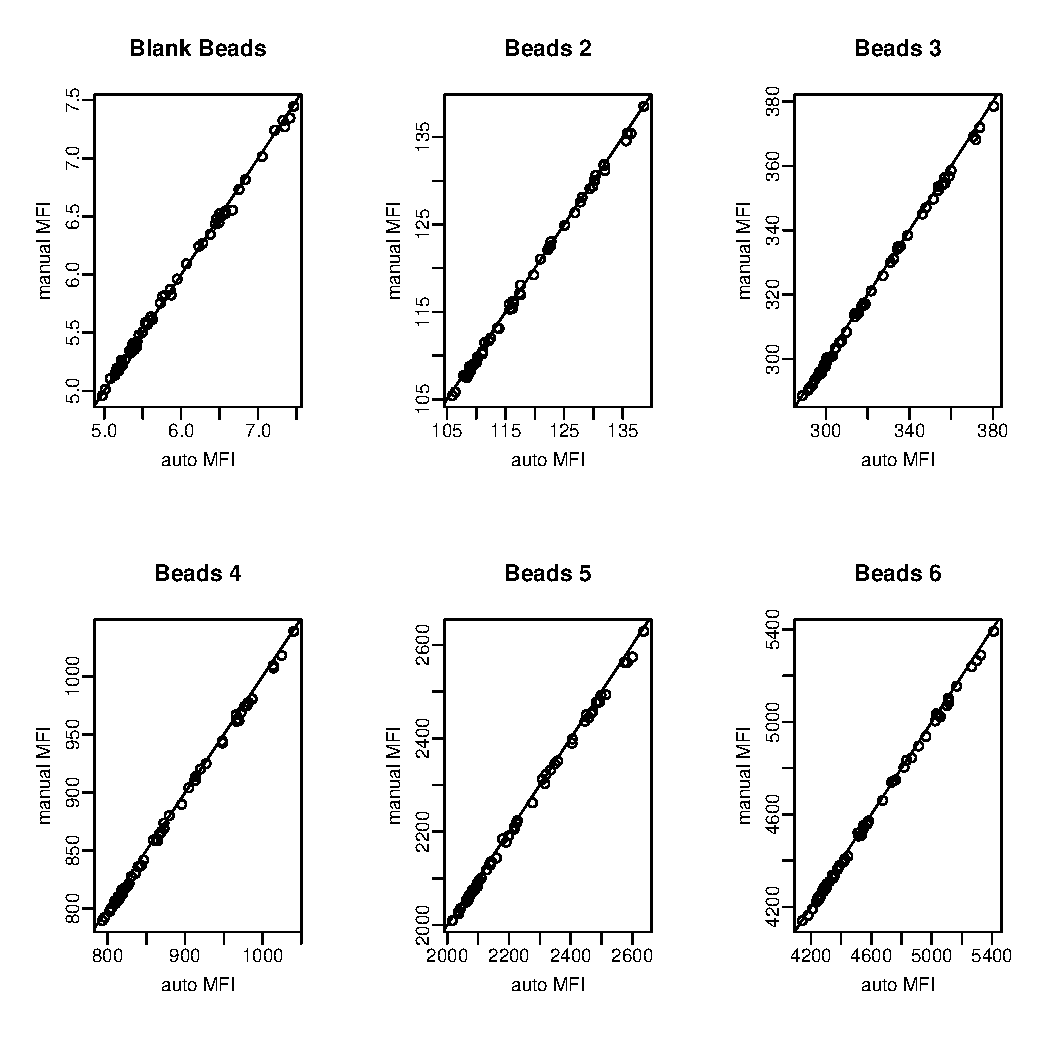
\includegraphics[scale=0.6]{IL2RA/figures/Beads/manual-auto-mfi.pdf}
\caption{
\label{figure:bead-agreement}
Agreement with manual.
}
\end{figure}



\begin{figure}[ht]
\centering
\begin{subfigure}[b]{.4\textwidth}
    \centering
    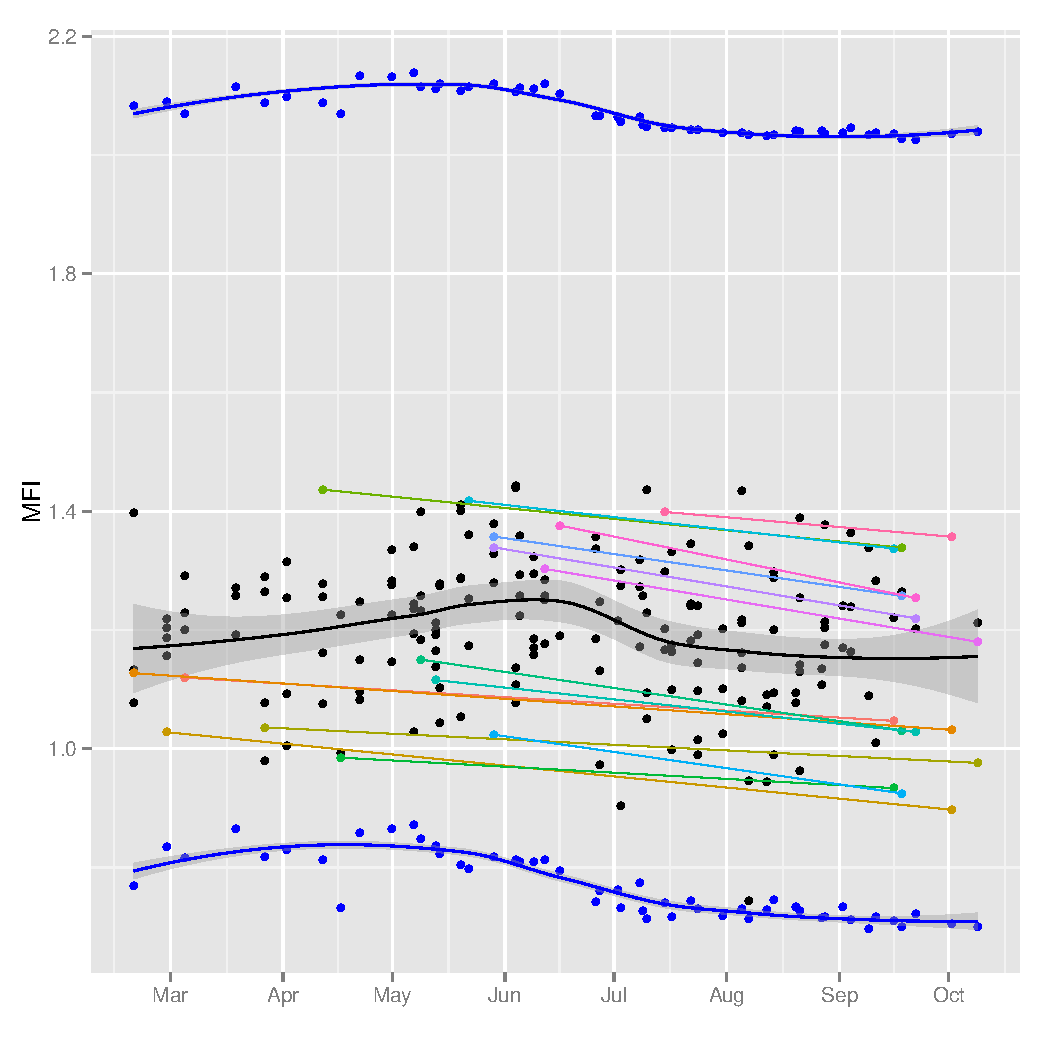
\includegraphics[scale=.3]{IL2RA/figures/CD25-MFI-time-effect-repeatability.pdf}
    \caption{Unormalised.}
\end{subfigure}
~
\begin{subfigure}[b]{.4\textwidth}
    \centering
    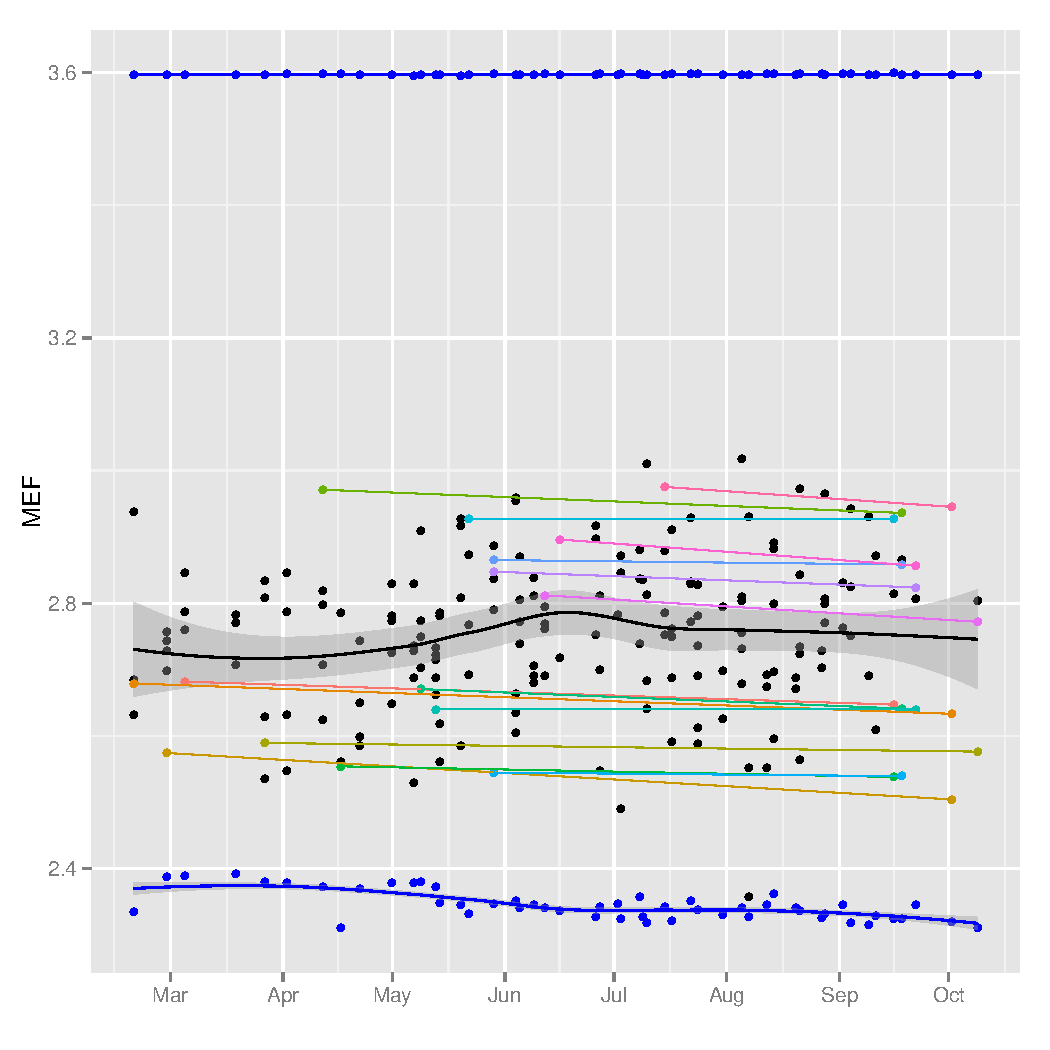
\includegraphics[scale=.3]{IL2RA/figures/CD25-MFI-time-effect-beads-normalised.pdf}
    \caption{Normalised}
\end{subfigure}
~
\begin{subfigure}[b]{.4\textwidth}
    \centering
    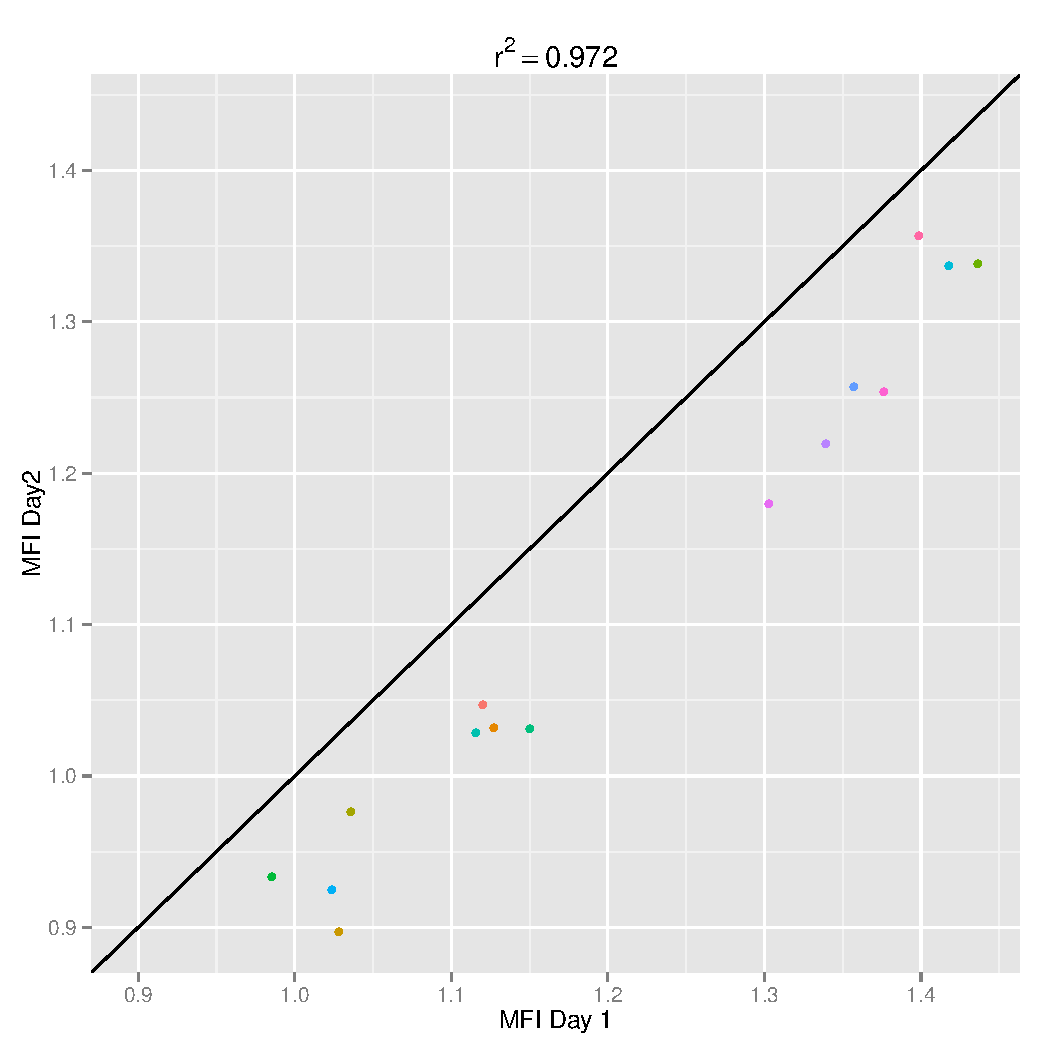
\includegraphics[scale=.5]{IL2RA/figures/CD25-MFI-repeatability.pdf}
    \caption{Unormalised: $r^2=0.629$}
\end{subfigure}
~
\begin{subfigure}[b]{.4\textwidth}
    \centering
    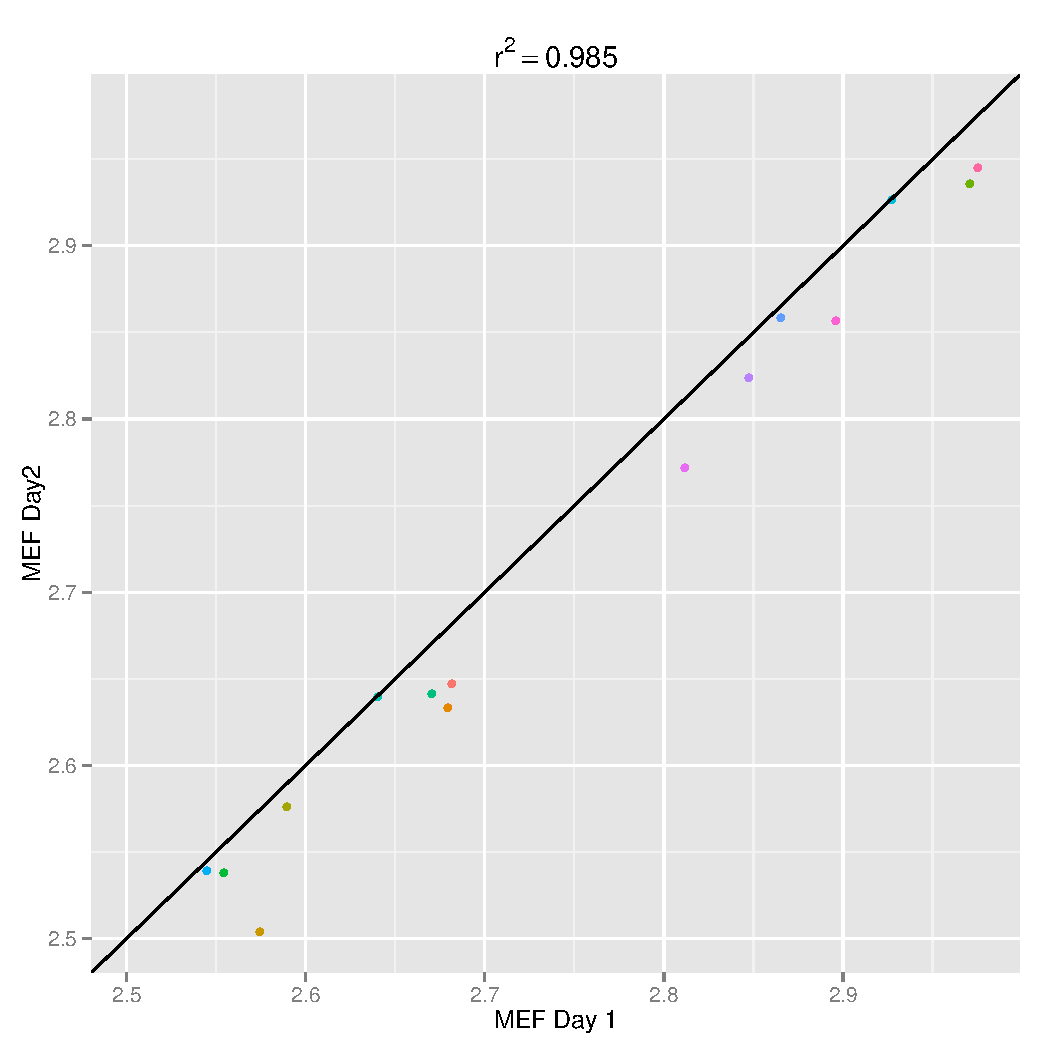
\includegraphics[scale=.5]{IL2RA/figures/CD25-MFI-beads-normalised.pdf}
    \caption{Normalised: $r^2=0.937$}
\end{subfigure}
\caption{
\label{figure:CD25-MFI-beads-normalised}
\textbf{Bead normalisation partially corrects for long term time effect in CD25 MFI of the memory cell population.}
In \textbf{(a)} and \textbf{(b)}, the blue points represent the MFIs of the bead populations, in black the MFIs of the memory cell populations.
A loess regression is fitted to the MFIs of the beads and memory cells.
The points joined by lines are MFIs from the $16$ recalled individuals (Table~\ref{table:IL2RA-recalled-individuals}).
The normalisation step involves aligning the peaks of the two bead populations across days to the overall mean of each of the populations (the dashed blue).
The normalisation improves the repeatability of the MFI in recalled individuals from $r^2=0.629$ \textbf{(c)} to $r^2=0.937$ \textbf{(d)}.
}
\end{figure}




%%% CD25POS
\section{Univariate Gating on CD25: Defining Thresholds on Naive Cells}

%The population of non regulatory CD4+ T cells is not clearly bimodal on CD25 like CD45RA.
The approach adopted by the manual method is to define a threshold above which cells are considered CD25 positive.
\citet{Dendrou:2009bl} select this threshold by using an isotype control.
%adjusted using the daily bead data.
This leads to a different gate position per sample per day (Figure~\ref{figure:cd25pos-gates}).
We notice that on some days there is greater variability in the positions on the gates.
Also we observe a downwards time-trend in the position of the gates which can be explained by
the gates needing to be moved to account for the sensitivity deterioration of the APC-CD25 channel of the
flow cytometer (Figure~\ref{figure:memory-CD25MFI-time-effect}).
This trend is also visible in \citet{Dendrou:2009bl}.

%As we can see from Figure~\ref{figure:mef}, the Memory T Cell MFI range is in between the MFI of the blank beads and dimmest bead population.
%Our automatic approach relies 
%Thus we define a threshold to distinguish CD25 positive from CD25 negative cells using the automatically gated bead data on the day which the sample was ran.
Isotype controls are a way of defining marker positivity based on a sample stained with non-specific antibodies
(antibodies which will not bind to the target we are interested in measuring).
Beside the disadvantage of wasting part of our sample for control purposes,
they are not necessarily an accurate measure of background fluorescence as
they are themselves a source of extra noise linked to differences in the constitution of the control sample,
the behaviour of the staining and other sources of technical variation.
On the other hand blank beads constitute a more stable reference which we can use to define an APC-CD25 threshold
provided we assume that the blank bead population represent the detection threshold of the instrument.
The threshold defined by my approach is set as the $95^{th}$ percentile of the automatically gated blank bead population on that day.
However because we only have one bead set per day this implies that we have a single fixed CD25 gate for all samples on that day.
The position of my automatic CD25 gates lie above the manual ones and so our gating is more stringent, returning
lower percentages of naive \protein{CD25}+ cells than reported by the manual approach (Figure~\ref{figure:cd25pos-gates}).

%In order to assess the dependency of the repeatability on the gates we chose the percentage phenotypes rather than the MEF.
%The concept of repeatability is explained in Appendix~\ref{repeatability}.
The automatic method for setting \protein{CD25} thresholds (\texttt{beads.auto}) shows improved repeatability of the percentage of \protein{CD25}+ naive T cell phenotype
than manual (Figure~\ref{figure:repeatability-cd25pos-naive}).
This is likely due to the decrease in variance in the automatically gated cell phenotype since the automatically defined threshold is higher than the manual one.
This improvement in repeatability translates into stronger association of the cell phenotype with genotype and sex (Table~\ref{table:naive-cd25pos-association}).

\clearpage

\begin{figure} [h]
\centering
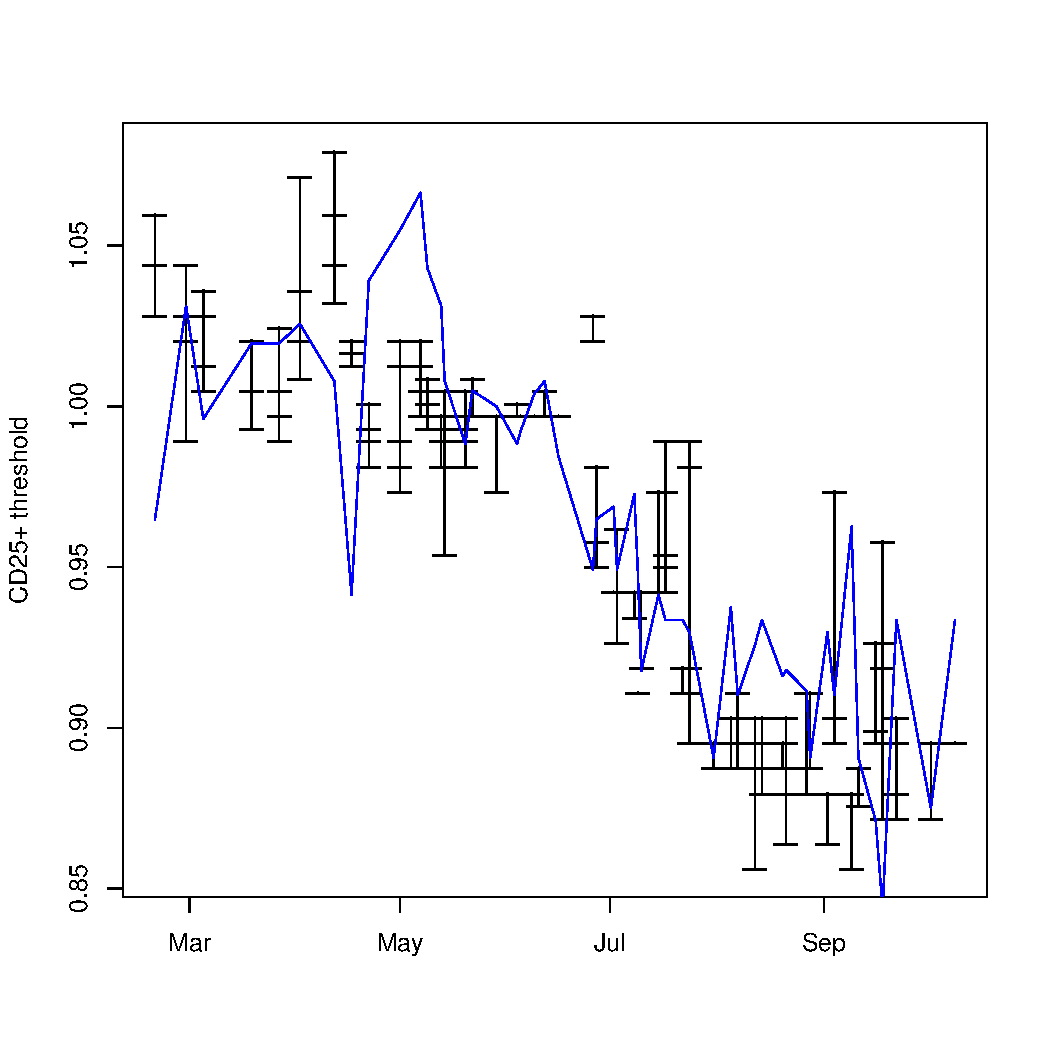
\includegraphics[width=.5\textwidth] {IL2RA/figures/cd25pos-gates.pdf}
\caption{
\label{figure:cd25pos-gates}
\textbf{Position of naive \protein{CD25}+ gate over duration of experiment.}
The black horizontal dashes are the positions of the manual CD25+ gates for all 195 samples over the time course of the experiment (51 days).
The vertical black lines represent the days and so define the range of the gate positions on a given day.
The blue line represents our automatic CD25+ gate which corresponds to the $95^{th}$ percentile of the blank bead population.
}
\end{figure}


\begin{figure}[h]
\centering
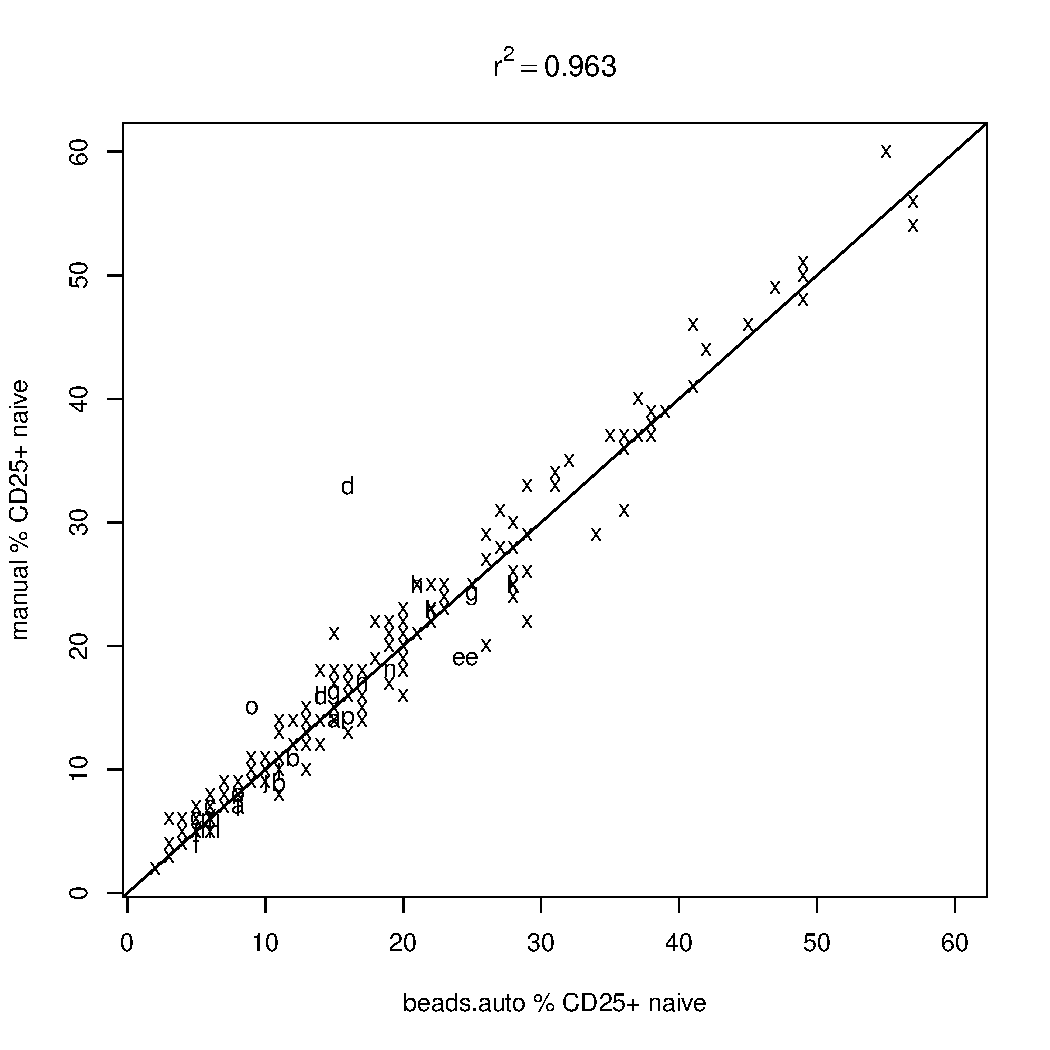
\includegraphics[width=.5\textwidth]{IL2RA/figures/Agreement/naive-cd25pos-beads-manual-agreement.pdf}
\caption{ 
\label{figure:threshold-manual-agreement}
\textbf{Agreement with manual of percentage of naive \protein{CD25}+ cell phenotype.}
Agreement of CD25 beads threshold method \texttt{beads.auto} with manual for percentage of CD25 positive naive cells.
Red points represent the $20$ samples where the cell phenotypes differ the most with manual 
whereas the green points represent the $20$ samples with the closest agreement.
Individual d is included in the bottom $20$.
}
\end{figure}


\begin{figure}[h]
\centering
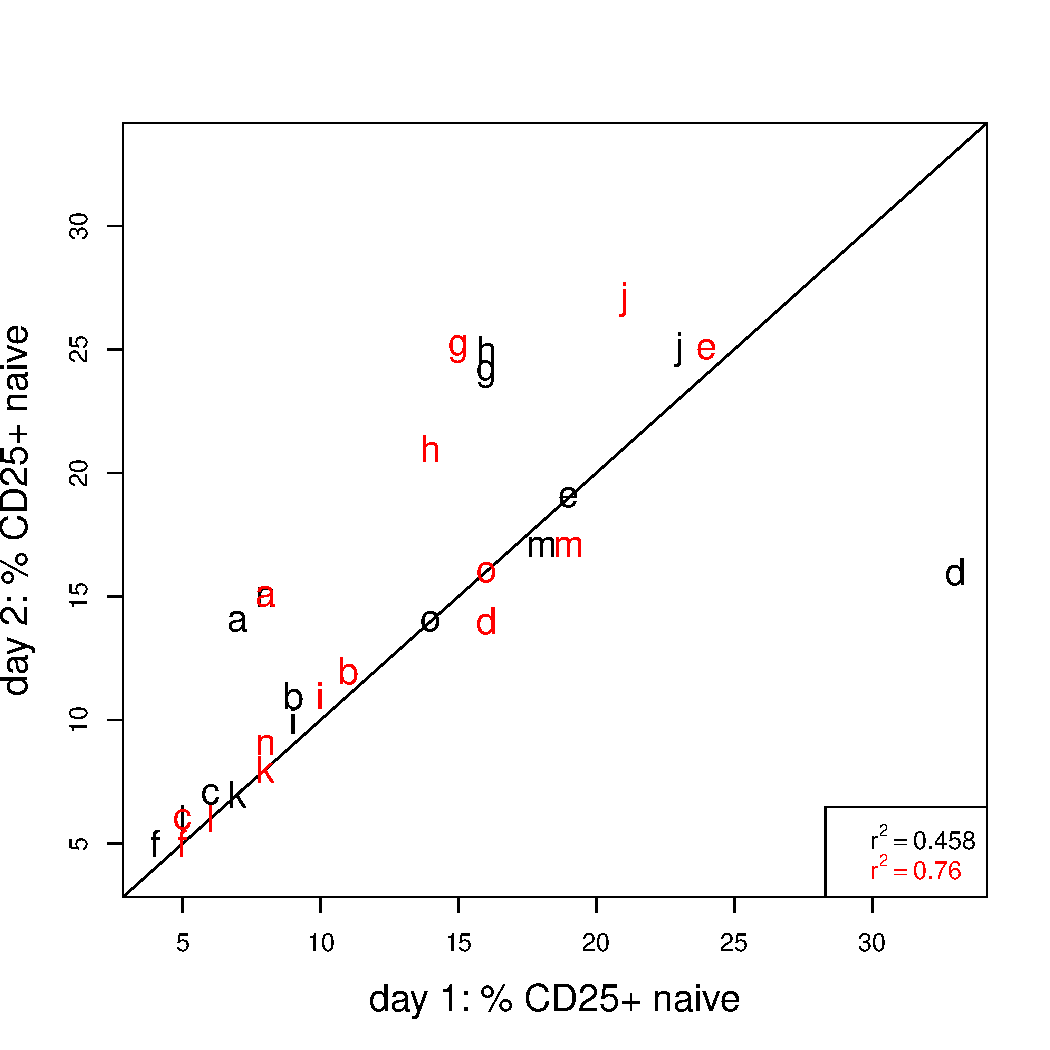
\includegraphics[width=.5\textwidth]{IL2RA/figures/repeatability-cd25pos-naive.pdf}
\caption{
\label{figure:repeatability-cd25pos-naive}
\textbf{Repeatability of percentage of naive \protein{CD25}+.}
Repeatability of the percentage of naive cells which are CD25 positive from day one to day two.
The overall repeatability of this cell phenotype was better with the beads based threshold than the manual one.
Letters are used to identify indidividuals see Table~\ref{table:IL2RA-recalled-individuals}.
$r^2$ is the Pearson correlation squared.
}
\end{figure}

\begin{table}[h]
\centering
\begin{tabular}{lrrr}
\rowcolor{Gray}
\snp{rs12722495} & effect & 95\%CI          & p-value\\
manual           & 0.172  & [-0.052;0.396]  & 0.1312672\\
beads.auto       & 0.312  & [0.079;0.546]   & \textcolor{red}{0.00905709}\\
\rowcolor{Gray}
\snp{rs2104286}  & effect & 95\%CI          & p-value\\
manual           & -0.481 & [-0.666;-0.296] & \textcolor{red}{7.9E-07}\\
beads.auto       & -0.528 & [-0.721;-0.335] & \textcolor{red}{2.2E-07}\\
\rowcolor{Gray}
\snp{rs11594656} & effect & 95\%CI          & p-value\\
manual           & -0.058 & [-0.227;0.111]  & 0.4987954\\
beads.auto       & -0.077 & [-0.255;0.101]  & 0.3947316\\
\rowcolor{Gray}
Age              & effect & 95\%CI          & p-value\\
manual           & 0.037  & [0.024;0.049]   & \textcolor{red}{2E-08}\\
beads.auto       & 0.037  & [0.024;0.05]    & \textcolor{red}{7E-08}\\
\rowcolor{Gray}
Sex              & effect & 95\%CI          & p-value\\
manual           & -0.217 & [-0.444;0.01]   & 0.06048679\\
beads.auto       & -0.253 & [-0.49;-0.016]  & \textcolor{red}{0.03687386}\\
\end{tabular}
\caption{
\label{table:naive-cd25pos-association}
\textbf{Genotype, age and sex effect sizes on percentage of \protein{CD25}+ cells.}
Effect of \snp{rs12722495}, \snp{rs2104286}, \snp{rs11594656}, age and sex,
on the percentage of \protein{CD25}+ naive cells.
}
\end{table}


%%% CD45RA
\section{Univariate Gating on CD45RA: Fitting Mixtures on Non T Regs}

The \protein{CD45RA} gating can be done by fitting a mixture of two univariate distributions to model the naive and memory cell populations.
In this section, we will only focus on the memory cell population.
%Generally non regulatory CD4+ T cells appear bimodal on CD45RA because it is known to be a marker lost upon activation of naive cells to memory cells.
To model this, we assume a mixture of two normally distributed populations (naive and memory cells) and we use the posterior probability of $95\%$ as
a cut-off to assign membership to \protein{CD45RA}- (memory) or \protein{CD45RA}+ (naive).
The posterior probability can be thought of as the confidence with which an event can be assigned to a cluster.
If the posterior probability is less than $95\%$ then the cells for both components, then these are not assigned to a cluster,
this is equivalent to the group of cells which fall in between the range defined by
the two CD45RA gates in manual gating and so considered to belong be neither truly naive nor memory,
but instead to be in a transitional state (Figure~\ref{figure:manual-gating-strategy}d).

We used the \Rpackage{mixtools} R package for analysing finite mixture models which provides an implementation of the EM algorithm \citep{Dempster:1977ul}
to fit Gaussian (\Rfunction{normalmixEM}) but also semi-parametric symmetric distributions (\Rfunction{spEMsymloc}).
%Returns semiparametric EM algorithm output (Bordes et al, 2007, and Benaglia et al, 2009) for location mixtures of univariate data and symmetric component density.
The initial estimate for the location of the two mixtures was given by running the K-medoids algorithm.
The EM algorithm is then run until convergence to to estimate the parameters.
%(see Appendix~\ref{EM}).
%Because we are only dealing with a mixture of two distributions only one mixing parameter needs to be estimated since the other is simply its complement.
%The other parameters to be estimated are the parameters of the distribution such as the mean and the variance when fitting a mixture of Gaussians or simply the location parameter
%for the semi-parametric distributions..
The parameters of the univariate Gaussian distribution are the mean (location) and the variance.
%More general distributions which are also symmetric
Semiparametric symmetric distributions are kernel density estimates centered around a location parameter.
The bandwidth parameter of the kernel density estimate is fixed to $0.1$ but could also have been estimated heuristically from the data.

The agreement with manual of the memory CD25 MEF is good since this cell phenotype is not very sensitive to the position of the \protein{CD45RA} gate (figure needed).
This translates in similar repeatability to that obtained with manual gating (Table~\ref{table:repeatability-memory-cell-MEF-phenotype}) and similar effect sizes
(Table~\ref{table:memory-cell-mef-effect}).

On the other hand, the repeatability of the percentage of memory cell phenotype is far more sensitive to the gating method.
We can see that both automatic mixture model approaches (\texttt{mm} and \texttt{sp.mm}) yield worse repeatability than manual (Figure~\ref{figure:repeatability-memory}).
As is the case for the sample from individual d on day one (Figure~\ref{figure:mm-memory}c),
the repeatability is compromised when the mixture of distributions approach fails to find a suitable gate because of poor model fit.
%As the same individual shows a very different profile on day two, I believe that, in this case, the noise is due to technical variation on that day rather
%than true biological variation.
%\subsection{Improved Repeatability when Averaging Gate Positions}
One reason why the manual gates on that day are more appropriate is because a human uses prior knowledge obtained from other samples of where the gates should lie.
This motivates borrowing information from other samples.
A first attempt at learning from other samples (\texttt{learned.mm}) is to compute the mean of the position of the CD45RA gates defined by the \texttt{mm}
method across all samples from the same day excluding the outlying sample from individual d on day one.
Similar to the threshold method for \protein{CD25}+ covered in the previous section, we now have a fixed gate for all samples analysed on the same day.
The \texttt{learned.mm} agreement with manual is improved over \texttt{mm} but not as good as \texttt{sp.mm}.
%but this time requires estimation of gate position by mm followed by averaging their position.
%When attempting to gate more noisy samples, a manual gater will maybe use other samples as a reference.
%One way of better gating is to use prior knowledge from other samples from the same day where the repeatability is good.
By decreasing the variance in gate position, this method improved overall repeatability (Figure~\ref{figure:repeatability-memory-learned})
but manual still achieves higher repeatability (Table~\ref{table:repeatability-results}) since it is better at dealing with outliers.
As we can see from the effect sizes in Table~\ref{table:memory-cell-pct-effect}, manual gating is able to detect \snp{rs12722495},
age and sex effects, whereas the automatic methods sometimes fail.

\clearpage

%% memory cell CD25 MEF
\begin{table} [h]
\centering
\begin{tabular} {|lc|}
\cline{1-2}
Method & $r^2$ \\
\cline{1-2}
manual     & 0.998 \\
mm         & 0.997 \\
sp.mm      & 0.998 \\
learned.mm & 0.998 \\
\cline{1-2}
\end{tabular}
\caption{  
  \label{table:repeatability-memory-cell-MEF-phenotype}
  \textbf{Repeatability of the CD25 MEF memory cell phenotype.}
  $r^2$ is the Pearson correlation squared.
}
\end{table}
\begin{table}[h]\footnotesize
\centering
\begin{tabular}{lrrr}
\rowcolor{Gray}
\snp{rs12722495} & effect  & 95\%CI            & p-value\\
manual     & 169.604 & [113.392;225.816] & \textcolor{red}{1.402171E-08}\\
mm         & 167.422 & [109.84;225.005]  & \textcolor{red}{4.185172E-08}\\
sp.mm      & 163.481 & [106.792;220.17]  & \textcolor{red}{5.274774E-08}\\
learned.mm & 166.335 & [109.324;223.346] & \textcolor{red}{3.792051E-08}\\
\rowcolor{Gray}
\snp{rs2104286} & effect  & 95\%CI            & p-value\\
manual     & -24.507 & [-71;21.987]      & 0.2996305\\
mm         & -23.494 & [-71.122;24.134]  & 0.331603\\
sp.mm      & -24.596 & [-71.486;22.293]  & 0.3019448\\
learned.mm & -24.226 & [-71.382;22.929]  & 0.3119814\\
\rowcolor{Gray}
\snp{rs11594656} & effect  & 95\%CI            & p-value\\
manual     & 5.832   & [-36.612;48.276]  & 0.786572\\
mm         & 3.996   & [-39.927;47.919]  & 0.8576929\\
sp.mm      & 6.422   & [-36.82;49.664]   & 0.7697717\\
learned.mm & 6.216   & [-37.271;49.703]  & 0.7781819\\
\rowcolor{Gray}
Age         & effect & 95\%CI         & p-value\\
manual     & -1.641 & [-4.735;1.453] & 0.2966789\\
mm         & -1.403 & [-4.573;1.767] & 0.3836938\\
sp.mm      & -1.442 & [-4.563;1.679] & 0.3629259\\
learned.mm & -1.577 & [-4.715;1.562] & 0.3227908\\
\rowcolor{Gray}
Sex        & effect  & 95\%CI           & p-value\\
manual     & -25.857 & [-82.84;31.126]  & 0.3717028\\
mm         & -20.922 & [-79.391;37.547] & 0.4809634\\
sp.mm      & -21.794 & [-79.356;35.768] & 0.4558872\\
learned.mm & -23.264 & [-81.153;34.624] & 0.4287351\\
\end{tabular}
\caption{
\label{table:memory-cell-mef-effect}
\textbf{Memory CD25 MEF effect sizes.}
Effect of \snp{rs12722495}, \snp{rs2104286}, \snp{rs11594656}, sex and age on memory CD25 MEF.
}
\end{table}


%% memory cell percentage 
\begin{figure}[h]
    \begin{subfigure}[b]{.5\textwidth}
        \centering
        \includegraphics[width=\textwidth]{IL2RA/figures/Agreement/mm-manual-agreement.pdf}
        %\caption{ Agreement of Gaussian mixture model method (mm) with manual for MEF and for memory percentage.}
       \caption{ }
        \label{figure:mm-manual-agreement}
    \end{subfigure}
    ~
    \begin{subfigure}[b]{.5\textwidth}
       \includegraphics[width=\textwidth]{IL2RA/figures/Agreement/sp-mm-manual-agreement.pdf}
       %\caption{ Agreement of semi-parametric mixture model method (sp.mm) with manual for MEF and for memory percentage.}
       \caption{ }
        \label{figure:sp-mm-manual-agreement}
    \end{subfigure}
    \caption{
    \label{figure:memory-percentage-agreement}
    \textbf{Agreement of percentage of memory cell obtained from \texttt{mm} and \texttt{sp.mm} with manual.}
    The agreement with manual is better for the more flexible semiparametric \texttt{sp.mm} approach (b) than for \texttt{mm} (a),
    though sample from individual d still remains an outlier.
    Red points represent the $20$ samples where the cell phenotypes differ the most with manual 
    whereas the green points represent the $20$ samples with the closest agreement.
    %Some of the red points for \texttt{mm} (\ref{figure:mm-manual-agreement}) are presented in Appendix~\ref{outliers}.
    }
\end{figure} 

\begin{figure}[h]
 \centering
 \includegraphics[scale=.6]{IL2RA/figures/Agreement/learned-mm-manual-agreement.pdf}
 %\caption{ Agreement of average daily gate positions of Gaussian mixture model method (learned.mm) with manual for MEF and for memory percentage.}
 \caption{
 \label{figure:learned-mm-manual-agreement}
 \textbf{Agreement of percentage of memory cell obtained from \texttt{learned.mm} with manual.}
 By taking the average of the gate positions on the day (\texttt{learned.mm}), we are able to gate sample d so that it is no longer an outlier
 as in Figure~\ref{figure:memory-percentage-agreement}.
 Red points represent the $20$ samples where the cell phenotypes differ the most with manual 
 whereas the green points represent the $20$ samples with the closest agreement.
  }
\end{figure} 

\begin{figure}[h]
\begin{subfigure}[h]{.5\textwidth}
   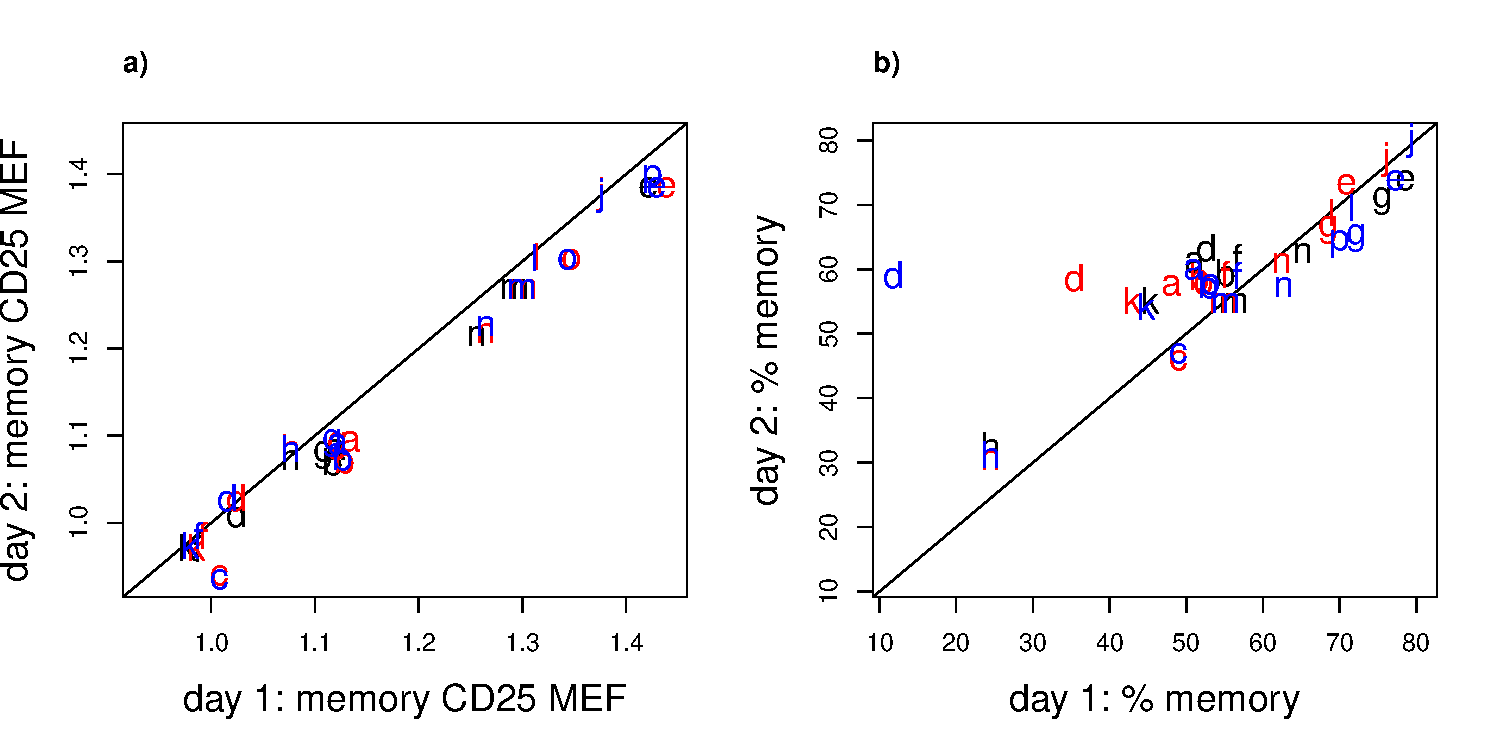
\includegraphics[width=\textwidth]{IL2RA/figures/repeatability-memory.pdf}
   \caption{}
   \label{figure:repeatability-memory}
\end{subfigure}
~
\begin{subfigure}[h]{.5\textwidth}
   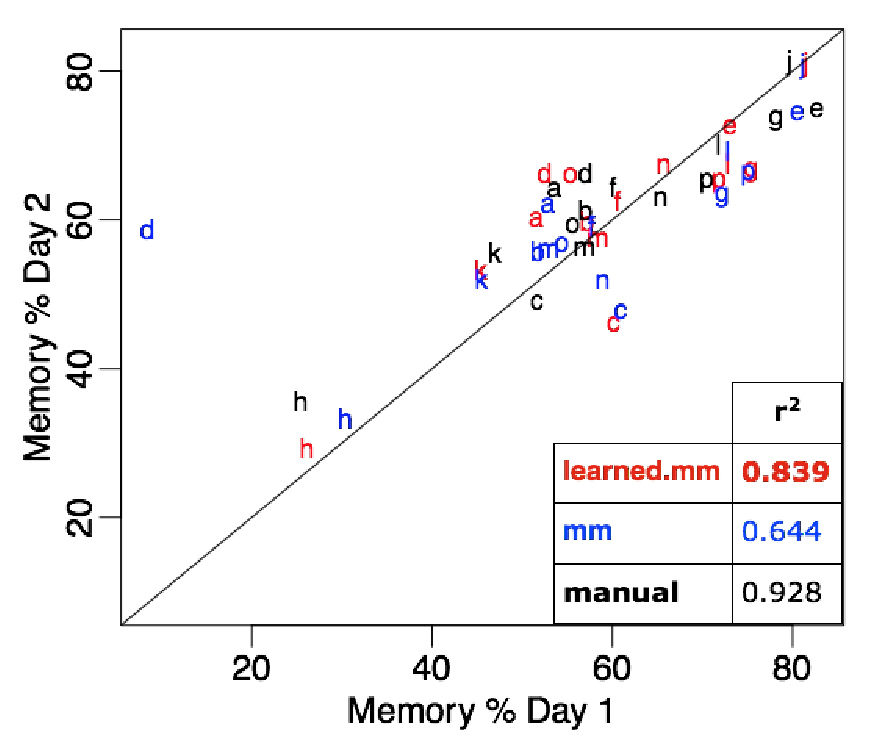
\includegraphics[width=\textwidth]{IL2RA/figures/repeatability-memory-learned.pdf}
   \caption{}
   \label{figure:repeatability-memory-learned}
\end{subfigure}
~
\begin{subfigure}[h]{\textwidth}
   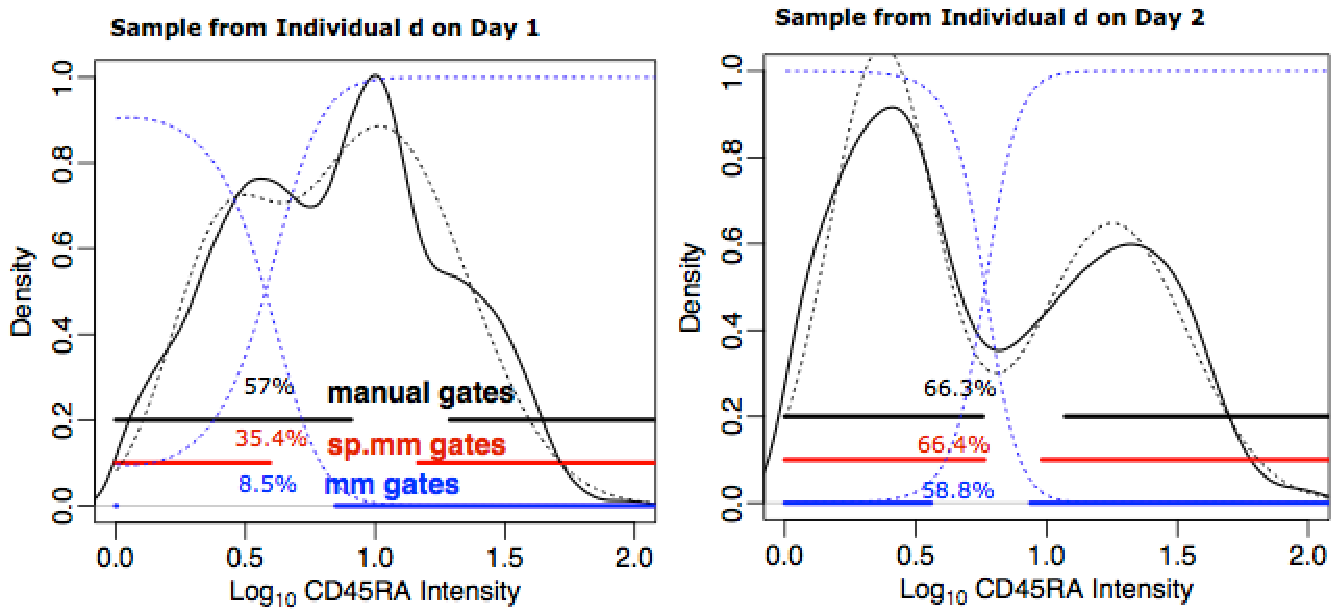
\includegraphics[width=\textwidth]{IL2RA/figures/mm-memory.pdf}
   \caption{}
   \label{figure:mm-memory}
\end{subfigure}
\caption{
\textbf{Repeatability of the percentage of memory cells phenotype.}
Semi-parametric mixtures (\texttt{sp.mm}) yields better repeatability than Gaussian mixture model (\texttt{mm}) but individual d remains a clear outlier (a).
The mixture model approach failed to return a sensible gate position for individual d on day one because the data does not fit the two component Gaussian mixture model (c).
The \texttt{learned.mm} approach improves on repeatability by more sensible gating on the outlier sample (b).
}
\end{figure}

\begin{table}[h]\footnotesize
\centering
\begin{tabular}{lrrr}
\rowcolor{Gray}
\snp{rs12722495} & effect  & 95\%CI            & p-value\\
 manual     & -0.036  & [-0.202;0.131]    & 0.6737116\\
 mm         & 0.046   & [-0.162;0.255]    & 0.662058\\
 sp.mm      & 0.038   & [-0.137;0.212]    & 0.6713971\\
 learned.mm & 0.036   & [-0.137;0.21]     & 0.6799432\\
\rowcolor{Gray}
\snp{rs2104286}  & effect  & 95\%CI            & p-value\\
 manual     & 0.086   & [-0.052;0.223]    & 0.2196305\\
 mm         & 0.066   & [-0.106;0.239]    & 0.4495351\\
 sp.mm      & 0.082   & [-0.063;0.226]    & 0.265578\\
 learned.mm & 0.094   & [-0.049;0.238]    & 0.1971427\\
\rowcolor{Gray}
\snp{rs11594656} & effect  & 95\%CI            & p-value\\
 manual     & 0.063   & [-0.063;0.188]    & 0.3255796\\
 mm         & 0.004   & [-0.155;0.163]    & 0.9591669\\
 sp.mm      & 0.035   & [-0.098;0.168]    & 0.6052556\\
 learned.mm & 0.034   & [-0.098;0.167]    & 0.6114843\\
\rowcolor{Gray}
Age         & effect & 95\%CI         & p-value\\
 manual     & 0.018 & [0.009;0.027] & \textcolor{red}{0.00014048}\\
 mm         & 0.009 & [-0.003;0.02] & 0.14226\\
 sp.mm      & 0.019 & [0.009;0.028] & \textcolor{red}{0.00018355}\\
 learned.mm & 0.016 & [0.007;0.026] & \textcolor{red}{0.00105886}\\
\rowcolor{Gray}
Sex         & effect & 95\%CI         & p-value\\
 manual     & 0.178   & [0.009;0.346]    & \textcolor{red}{0.0389072}\\
 mm         & 0.162   & [-0.05;0.373]    & 0.1335836\\
 sp.mm      & 0.15    & [-0.027;0.326]   & 0.09721186\\
 learned.mm & 0.212   & [0.036;0.389]    & \textcolor{red}{0.01860495}\\
\end{tabular}
\caption{
\label{table:memory-cell-pct-effect}
\textbf{Memory percentage effect sizes.}
Effect of \snp{rs12722495}, \snp{rs2104286}, \snp{rs11594656}, sex and age on memory cell percentage.
}
\end{table}





%%% DISCUSSION
\section{Discussion}

%A more real challenge however is to do with the nature of flow data.
%Noise or unexplained variation is inherent to all technologies and the signal to noise ratio in flow cytometry can vary greatly depending on the sample,
%the experimental protocol and the instrument.
%Even when running a "clean" sample such as beads which are manufactured to be identical on a well calibrated instrument the signal to noise ratio of the resulting bead populations is never greater than 30.
%In biological samples the level of noise is much higher and so is the number of outliers which contribute to confusing automatic methods,
%especially when in most cases the number of clusters is unknown and needs to be estimated from the ratio of explained to unexplained variance in the data.
%Many clustering solutions have been suggested as part of the Bioconductor suite of packages which adopt different approaches to trying to solve this problem.
%But remains the problem of how to benchmark these various solutions: comparison to manual gating, correlation with clinical outcome?
%One criteria we have suggested and tested is that of repeatability of results derived from stable features in samples from the same healthy individual recalled up to 7 months later. (Spidlen et al., 2010).
%
In this chapter, I have shown that bead data is readily gated by automatic methods and that the results are comparable to manual gating.
Automatic gating of bead data is fast and automates other related tasks such as MFI to MEF transformation
and reporting of instrument properties such as the detection threshold or the signal-to-noise ratio (or coefficient of variation).

Gating of biological data is more difficult as we have little prior knowledge of the sample we are analysing.
So far, we have developed two automatic univariate gating strategies:
\begin{itemise}
\item a bead defined threshold method on \protein{CD25} to identify CD25+ naive cells
\item a two component mixture model on \protein{CD45RA} to identify memory cells
\end{itemise}

My \protein{CD25} univariate gating method (\texttt{beads.auto}) relies on defining a threshold based on automatically gated bead data.
The percentage of naive \protein{CD25}+ cells phenotype identified with my approach showed better repeatability than manual (Figure~\ref{figure:repeatability-cd25pos-naive}).
My approach defines one threshold for all samples gated on the same day which seems appropriate given the blank bead population
yields the detection threshold of the instrument on that day.
The manual approach, which relies on isotype controls, allows for different thresholds per day.
Isotype controls should theoretically be an estimate of background but have been criticised for being an extra source of noise \citep{OGorman:1999vd}.
Because the CD25 thresholds obtained by my method are higher than the manual ones, our estimated percentage of 
CD25+ naive cells is lower.

My \protein{CD45RA} univariate gating method fits a specific model to the data: a mixture of two univariate distributions.
The parameters of these distributions are estimated using the EM algorithm \citep{Dempster:1977ul}.
The gates are defined as the thresholds at which the posterior probability or responsibility reaches \SI{95}{\percent}.
This represents a hard threshold to emulate manual gating.
%In the future it may be interesting to use all cells and average over the posterior probabilities.
However, if the model does not fit the data then it is unlikely that the position of the gate will be sensible,
which may give rise to outliers.

I used two benchmarks to evaluate my univariate gating strategies: repeatability and comparison of the effects sizes obtained 
by \citet{Dendrou:2009dv} using manual.

Repeatability is an independent measure which does not require comparison to other gating methods (such as manual).
Unfortunately, given that in our data set only 15 samples are repeated, it is difficult to evaluate methods on such a small sample size.
Moreover, good repeatability does not necessarily imply that the gating is correct but rather that the gating is consistent.
Hence repeatability, needs to be complemented with some metric, in the form of manual gating or some prior biological knowledge, to assess whether the computed cell phenotypes are in a sensible range.

We have seen how the difference in the identification cell phenotypes by different gating methods, greatly influences the estimated effect sizes.
In particular, outliers have an important influence depending on their leverage.
For example when testing association with age, outlier cell phenotypes from younger or older individuals have more leverage than ones closer to the mean.

%\paragraph{Outlier Detection Metric}
Hence, if we are to deploy automatic gating techniques more generally, detection of outliers is crucial.
We therefore require outlier detection metrics which do not only rely on the availability of repeated samples or manual gates.
For example, one metric of evaluating how well a model fits the data could be a cost function like the Mean Integrated Square Error (MISE).
We will expound on outlier metrics in later chapters.

When outliers have been detected, we may want to exclude these from the analysis or modify our gating method to account for these.
One simple way of modifying the method, is to use the gate positions in non-outlier samples to influence those in outliers.
%This clearly rests on the assumption that in the majority of samples, the position of the gate is correct.
I tried this approach with \texttt{learned.mm} by averaging gates on non-outlier samples and applying these to the outlier samples.
%thus exploiting day effects
A more formal approach could be to extend this by using some outlier metric to define weights so that \texttt{learned.mm} leans more heavily
towards samples where the model fits better.
%We have seen that one way of improving overall gating is to allow for the gate positions on well-gated samples to influence those of badly-gated ones.
Clearly, the implicit assumption with \texttt{learned.mmm} is that there are enough well-gated samples to positively influence the gate position of the ill-gated ones.
However, one may argue that this approach, conceals rather than addresses the underlying problem of poor model fit.
For example as we see from the trimodal distribution in Figure~\ref{figure:mm-memory}), we want to fit a three component instead of two component mixture model on this sample.

%\paragraph{Discovering New Subsets of Interest with Automatic Methods}
%So far in this chapter, I have only considered the cell phenotypes defined by \citet{Dendrou:2009dv}.
%In general, these cell populations may not necessarily represent true clusters but are established cells of interest within the field of immunology
%which are known to express \protein{CD25} and hence hypothesised to associate with \gene{IL2RA} SNPs.
%Potentially, there might exist other \protein{CD25} cell phenotypes than the ones under study which also correlate well with these SNPs.
%These might only be separable in higher dimensional space.
%These could be identifiable using unsupervised methods which find clusters in one or more dimensions when the number of clusters is unknown.
%Similar work has been undertaken by \citet{Aghaeepour:2012fq} in identifiying novel subsets which correlate with a clinical outcome in HIV patients.
%Fealect (?) is a method of choosing features of these cells subsets which best correlate with the response variable.

%\paragraph{An Internal Automatic Pipeline}

So far, MFI to MEF using beads has been automated but there are still many parts of the process which can be automated.
In later chapters, I will develop a modular pipeline to further automate the analysis of flow cytometry data generated by our lab.
It will be possible to plug in different types of transformations and gating strategies and see how this influences
the results of the analysis.
This should encourage the wider use of automatic analysis methods for flow data within our lab.


%The pipeline will be configurable to so account for the wealth Obviously the type of analysis will be dependent on the experiment but it may be possible 
%One of the reasons for this is simply that the analysis requirements for different types of flow experiments are so varied that it is difficult to design a solution which will service all needs.


